\documentclass[tikz]{standalone}
\usetikzlibrary[arrows,shapes]
\begin{document}
% Start of code
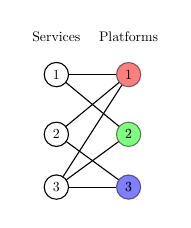
\begin{tikzpicture}[>=latex',join=bevel,scale=0.5,transform shape]
%%
%%
\definecolor{c1}{rgb}{0.70,0.25,0.25}%
\definecolor{c2}{rgb}{0.25,0.70,0.25}%
\definecolor{c3}{rgb}{0.25,0.25,0.70}%
%
\begin{scope}
  \pgfsetstrokecolor{black}
  %\draw[thick,red] (4bp,51bp) -- (4bp,191bp) -- (46bp,191bp) -- (46bp,51bp) -- cycle;
  \draw (25bp,185bp) node {Services};
\end{scope}
\begin{scope}
  \pgfsetstrokecolor{black}
  %\draw[thick,blue] (56bp,51bp) -- (56bp,191bp) -- (98bp,191bp) -- (98bp,51bp) -- cycle;
  \draw (77bp,185bp) node {Platforms};
\end{scope}
	\node (1) at (25bp,158bp) [draw,circle] {$1$};
  \node (2) at (25bp,115bp) [draw,circle] {$2$};
  \node (3) at (25bp,77bp) [draw,circle] {$3$};
  \node (4) at (77bp,158bp) [draw,circle,fill=red,opacity=0.5] {$1$};
  \node (5) at (77bp,115bp) [draw,circle,fill=green,opacity=0.5] {$2$};
  \node (6) at (77bp,77bp) [draw,circle,fill=blue,opacity=0.5] {$3$};
  \path[] (1) edge (4);
  \path[] (1) edge (5);
  \path[] (2) edge (4);
  \path[] (2) edge (6);
  \path[] (3) edge (4);
  \path[] (3) edge (5);
  \path[] (3) edge (6);
  \draw (77bp,158bp) node {$1$};
  \draw (77bp,115bp) node {$2$};
  \draw (77bp,77bp) node   {$3$};

\end{tikzpicture}
% End of code
\end{document}